% class options:
% - select either [german] or [english]
% - select the type of thesis from:
%   [bachelor, master, generic]
%   (in case of generic, use \type{} to specify it)
% - use option "alpha" for abbreviated citation (instead of numbers)
% - option "draft" is available, too
% - use options "utf8" or "latin1" to select inputencoding
\documentclass[german, bachelor, utf8, alpha]{thesis_KBS}

\usepackage{units}    % useful for settings units:              \unit[23]{m}
\usepackage{nicefrac} % for setting fractions esp. within text: \nicefrac{km}{h}
\usepackage{minted}
\usepackage{graphicx}
\usepackage{amsmath}
\usepackage{wrapfig}

\usepackage{algorithm, algorithmic}  % for pseudo code (cf. documentation)
\renewcommand{\algorithmiccomment}[1]{\qquad{\small // \textit{#1}}}

%%%%%%%%%%%%%%%%%%%%%%%%%%%%%%%%%%%%%%%%%%%%%%%%%%%%%%%%%%%%%%%%%%%%%%%%%%%%%%%

\begin{document}

\title{Prozedurale Modellierung von Schneedecken}
\author{Manuel Schwarz}
\email{manschwa@uni-osnabrueck.de}
\firstSupervisor{Prof. Dr. Oliver Vornberger}
\secondSupervisor{Prof. Dr. Sigrid Knust}
%\dept{...}                             % by default MI UOS
%\submitdate{November 2004}             % by default current month & year
%\signcity{}                            % by default Osnabr�ck
%signline{Osnabr�ck, 11. Dezember 2004} % by default "signcity, submitdate"

\generatetitle

\cleardoublepage

\begin{prefacesection}{Zusammenfassung}
Die vorliegende Arbeit entstand in der Arbeitsgruppe Medieninformatik an der
Universit"at Osnabr"uck im Bereich Computergrafik und besch"aftigt sich mit
prozeduraler Modellierung.
Kern der Arbeit ist die Generierung von Schneedecken zur naturgetreueren
Repr"asentation von Wetterverh"altnissen basierend auf Wetterdaten.
Diese werden mit Hilfe eines angen"ahrten Modells
und der Verwendung des sogenannten Marching Cubes Algorithmus realisiert.

\end{prefacesection}

\cleardoublepage
\tableofcontents
\cleardoublepage
\listoffigures


\startTextChapters %%%%%%%%%%%%%%%%%%%%%%%%%%%%%%

\chapter{Einleitung}

Diese Arbeit befasst sich mit dem Entwurf, der Konzeption und der Entwicklung
einer Methode zur Repr"asentation von Schneedecken.

\section{Motivation}

Im Rahmen der Masterprojektgruppe ''Virtueller Campus'' an der Universit"at
Osnabr"uck im Sommersemester 2011 sowie Wintersemester 2011/12.


\section{Zielsetzung}

Ziel der Arbeit ist es eine richtige Schneedecke mit Hilfe prozeduraler
Modellierung zu generieren und somit eine naturgetreuere Wetterdarstellung zu
gew"ahrleisten.\\
Insbesondere stehen hierbei die Algorithmen zur zur Modellierung der Schneedecke
im Vordergrund und weniger die Visualisierung.\\

\section{Aufbau der Arbeit}

Zun"achst wird eine kurze Einf"uhrung in das Thema Prozedurale Modellierung
gegeben. Diese beinhaltet die Entstehung, sowie den Boom Mitte der 80er Jahre
sowie die Entwicklung bis heute.\\
Darauf folgen einige grundlegende Konzepte und Ideen deren Theorie erl"autert
wird. Im Kapitel Umsetzung werden diese Konzepte Implementiert und angewendet.
Besonders im Fokus stehen hier der ins 3-dimensionale "ubertragene Punkt in
Polygon- sowie der Marching Cubes Algorithmus.



%%%%%%%  GRUNDLAGEN  %%%%%%%%

\chapter{Grundlagen}

Im folgenden Kapitel sollen die dieser Arbeit zugrunde liegenden theoretischen
Grundlagen aufgef"uhrt und erkl"art werden, bevor sie im Kapitel Umsetzung
implementiert werden.

\section{Prozedurale Modellierung}

Zu Beginn soll der Begriff der prozeduralen Modellierung n"aher beleuchtet
werden.

\section{Displacement Mapping}
\label{sec:displacement_mapping}

Das Displacement-Mapping geht aus dem Bump-Mapping hervor und stellt eine
Erweiterung dessen dar.\cite[S. 9]{texturing} Robert L. Cook beschreibt das
Displacement-Mapping erstmals 1984.\cite{displacement_mapping}

\begin{wrapfigure}{r}{0.4\textwidth}
    \vspace{-20pt}
    \begin{center}
        \includegraphics[width=0.35\textwidth]{pictures/displacement_mapping.jpg}
    \end{center}
    \vspace{-10pt}
    \caption[Beispiel f"ur Displacement Mapping]{Beispiel f"ur Displacement Mapping \cite{displacement_mapping_pic}}
    \label{fig:displacement}
    \vspace{-20pt}
\end{wrapfigure}

Dabei werden Texturen dazu benutzt die Objektoberfl"ache zu alternieren.
Das hei\ss t, es werden nicht nur die Normalen, wie beim
Bump Mapping ver"andert um eine gew"unschte Erscheinung der Oberfl"ache zu
simulieren\cite{bump_mapping}, sondern es wird die tats"achliche
Objektgeometrie modifiziert.
Dies geschieht, indem die Vertices eines Objekts anhand der Werte einer
Displacement-Map entlang der Normalen (senkrecht zur Oberfl"ache) verschoben
und die Normalen entsprechend angepasst werden.



In der Abbildung \ref{fig:displacement} ist ein
Beispiel f"ur eine solche
Displacement-Map und die Auswirkung auf die Oberfl"ache (Mesh) gegeben.
Die Displacement-Map enth"alt dabei Farbwerte von schwarz (keine Ver"anderung)
bis wei\ss (maximale Verschiebung des Vertex in Richtung der Normalen).
Im dritten Bild ist die ver"anderte Silhouette der Oberfl"ache gut zu erkennen.
Da bei dieser Vertexverschiebung auch die Normalen neu berechnet werden
sieht das Displacement-Mapping oftmals dem Bump-Mapping sehr "ahnlich, mit dem
entscheidenen Unterschied, dass die Struktur, die durch das Displacement-Mapping
erzeugt wird im Umriss des Objekts sichtbar ist.


\section{Punkt in Polygon - Algorithmus}
\label{sec:pip_theo}

Der Punkt in Polyon - Algorithmus ist ein Verfahren um festzustellen, ob ein
gegebener Punkt in einer Ebene innerhalb oder au\ss erhalb der Grenzen
eines Polygons liegt. Diese Methode findet vorwiegend Anwendung beim
Verarbeiten geometrischer Daten, wie zum Beispiel in der Computergrafik.\\
Bereits 1974 wurden zwei Ans"atze zur L"osung des Punkt-in-Polygon-Problems
f"ur nicht-konvexe Polygone
(Ray-Casting und Winkelsummation) vorgestellt.\cite[S. 13f.]{point_in_polygon}
In dem Artikel von Sutherland wird der Algorithmus dazu verwendet festzustellen
welche Oberfl"achen einer Szene n"aher am Betrachter liegen und welche
durch andere verdeckt werden.
\\
Im Folgenden wird n"aher auf das Konzept des Ray-Castings eingegangen, welches
in Abbildung \ref{fig:pip} illustriert wird.


\begin{figure}[htbp]
    \centering
    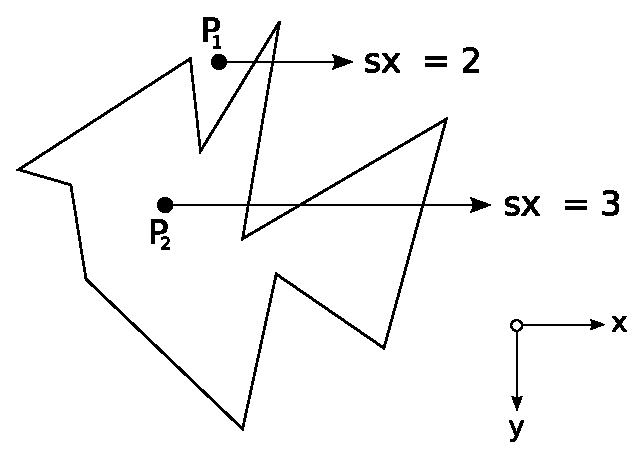
\includegraphics[width=250px]{pictures/punkt_in_polygon.eps}
    \caption{Punkt in Polygon Algorithmus}
    \label{fig:pip}
\end{figure}

Punkte werden getestest, indem man einen imagin"aren ''Strahl'' in eine
beliebige Richtung schickt und die Schnittpunkte mit den Kanten des Polygons
z"ahlt. Ist die Anzahl der Schnittpunkte gerade, so liegt der Punkt
au\ss erhalb, ist sie ungerade, so liegt der Punkt innerhalb des Polygons.\\
Um konsistente Ergebnisse zu erhalten falls ein oder mehrere Polygon-Vertices
genau auf dem Test-Strahl liegen, ist es notwendig die Sonderf"alle zu
betrachten, die in Abbildung \ref{fig:sonderfaelle} dargestellt sind.

\begin{figure}[htbp]
    \centering
    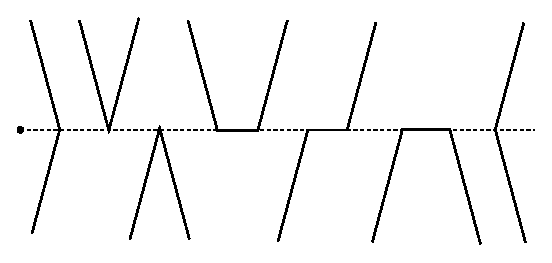
\includegraphics[width=300px]{pictures/sonderfaelle.eps}
    \caption{Sonderf"alle des Punkt in Polygon Algorithmus}
    \label{fig:sonderfaelle}
\end{figure}

Die Umgehung dieses Problems liegt in der Annahme, dass der Plygon-Vertex
infinitisimal "uber dem Test-Strahl liegt. Durch dieses Vorgehen wird
zus"atzlich festgelegt, zu welchem Polygon ein Pixel geh"ort, sollten
zwei Polygone einen oder mehrere Vertices gemeinsam haben.
\cite[S. 51ff.]{skript_cg}

\section{Marching Cubes - Algorithmus}
\label{sec:mc_theo}

%Der MC geht auf Lorensen und Cline zur"uck...
\subsection{Bedeutung}
Der Marching Cubes Algorithmus wurde im Jahr 1987 im Auftrag der General
Electric Company von Lorensen und Cline entwickelt, um ein effizienteres
Verfahren zur Visualisierung medizinischer Messdaten bereitzustellen.
\cite{marching_cubes}
Dabei wurde bis zum damaligen Zeitpunkt meist auf 2-dimensonale Bilddaten
von bildgebenden
Verfahren wie zum Beispiel der Computertomografie (CT) oder der
Magnetresonanztomografie (MRT) zur"uckgegriffen.
Da das Analysieren und Interpretieren dieser 2-dimensionalen Bilder
(Scheiben oder Schichten) besondere Schulung und Erfahrung bedarf, bietet der
Marching Cubes
Algorithmus eine aussagekr"aftige, 3-dimensionale Repr"asentation der
evaluierten Messdaten zur
Unterst"utzung von Medizinern in den unterschiedlichsten Bereichen.\\
Die vom CT bzw. MRT erzeugten Volumendaten liegen in Form von Voxel-Datenmengen
vor. Das hei\ss t, dass in regelm"a\ss igen Abst"anden die Dichte des Materials
ermittelt und gespeichert wird, wodurch ein gleichm"a\ss iges 3-dimensionales
Datengitter generiert wird. Die Nachteile eines solchen Modells sind der enorme
Speicherbedarf und die langsame Visualisierung im Vergleich zu einfachen
Drahtgittermodellen.\\
Der Marching Cubes Algorithmus erm"oglicht nun die zuvor genannten
Voxel-Datenmengen durch ein polygonales Oberfl"achenmodell anzun"ahren und somit
effizient zu visualisieren.


\subsection{Funktionsweise}
Der Marching Cubes Algorithmus verfolgt einen Divide-and-Conquer-Ansatz.
Um die gegebenen Volumen-Daten zu Triangulisieren betrachtet man zun"achst zwei
benachbarte bzw. direkt "ubereinanderliegende Schichten oder Ebenen. In einem
n"achsten Schritt werden vier benachbarte Voxel auf der unteren Ebene
\texttt{z} so
miteinander verbunden, dass sie ein Quadrat ergeben. Danach bilden diese mit
den genau dar"uberliegenden Voxeln der Ebene \texttt{z+1} einen imagin"aren
W"urfel (siehe Abbildung \ref{fig:mc}).

\begin{figure}[htbp]
    \centering
    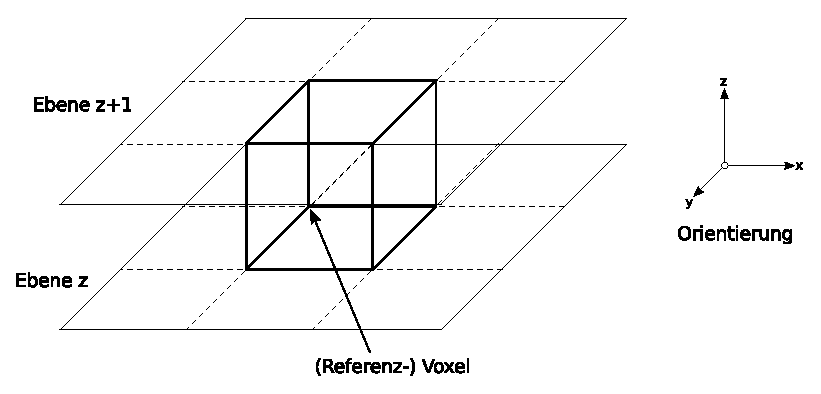
\includegraphics[]{pictures/marching_cube.eps}
    \caption{Marching Cube}
    \label{fig:mc}
\end{figure}

Dabei gibt es meist einen Referenzvoxel von dem aus die restlichen
Kubusecken mit Hilfe eines Offsets bestimmt werden.\\
Damit anschlie\ss end eine Oberfl"ache generiert werden kann wird wird f"ur
jeden Eckpunkt
gepr"uft, ob dieser innerhalb oder au\ss erhalb des betrachteten Objektes liegt,
was anhand der Dichtewerde bestimmt werden kann.
Liegen alle Eckpunkte innerhalb oder au\ss erhalb, so muss dieser W"urfel nicht
weiter untersucht werden und es wird zum N"achsten ''marschiert''.
Liegt hingegen ein Schnittpunkt des Kubus mit der Objektoberfl"ache vor, so
teilt diese den Marching Cube unweigerlich in Innen- und Au\ss enbereiche auf.\\
Da der W"urfel acht Eckpunkte besitzt und jeder Eckpunkt zwei Zust"ande
haben kann, gibt es genau $2^8 = 256$ M"oglichkeiten den Kubus zu zerteilen.
Aus Symmetriegr"unden k"onnen diese 256 F"alle auf die in Abbildung
\ref{fig:mc_possibilities} dargestellten 15 reduziert
werden.

\begin{figure}[htbp]
    \centering
    \includegraphics[width=310px]{pictures/marchingCubes.png}
    \caption[Marching Cube - Schnittm"oglichkeiten]
        {Marching Cube - Schnittm"oglichkeiten \cite{mc_possibilities}}
    \label{fig:mc_possibilities}
\end{figure}

Sind schlie\ss lich die Zust"ande aller beteiligten Voxel bestimmt, so wird in
einer Tabelle, der sogenannten
\texttt{TriangleLookupTable} nachgesehen, welche Dreiecke in dem vorliegenden
Fall gezeichnet werden m"ussen. Genauer gesagt, werden die W"urfelkanten
bestimmt, die von der Oberfl"ache geschnitten werden und wo auf den Kanten
die Eckpunkte der zu zeichnenden Dreiecke liegen.
In dem Kapitel \ref{sec:mc_algo} wird dieses Verfahren und die \texttt{TriangleLookupTable}
genauer erl"autert.\\
Wahlweise k"onnen f"ur eine bessere Ann"aherung an das Ursprungsobjekt die
Oberfl"achenpunkte entsprechend interpoliert werden. Ansonsten wird f"ur die
Berechnung der Dreiecke immer von der Mitte einer W"urfelkante ausgegangen.
Zur besseren Darstellung (Beleuchtung) lassen sich daraufhin die
Einheitsnormalen berechnen.\\
Ein Beispiel f"ur die Visualisierung eines aus 150 Schichten bestehenden
MRT-Modells soll die Abbildung \ref{fig:mc_head} geben, in der die
Ann"aherung an einen Kopf deutlich zu erkennen ist.

\begin{figure}[htbp]
    \centering
    \includegraphics[width=250px]{pictures/marching_cubes_head.png}
    \caption[Marching Cubes - Polygonmodell eines Kopfes]
        {Marching Cubes - Polygonmodell eines Kopfes \cite{mc_head}}
    \label{fig:mc_head}
\end{figure}




%%%%%%%  UMSETZUNG  %%%%%%%%

\chapter{Umsetzung}

%%%% TODO evtl. umschreiben, oder weglassen
%Dieses Kapitel besch"aftigt sich mit der Umsetzung und Implementierung der
%vorher genannten Konzepte. Nach einer Darstellung verschiedener
%L"osungsans"atze wird genauer auf den gew"ahlten Ansatz eingegangen.
%Besonders herausgestellt werden der Punkt in Objekt Algorithmus sowie der
%Marching Cubes Algorithmus, die den Kern dieser Arbeit darstellen.


\section{Ans"atze}

Dieses Kapitel befasst sich mit m"oglichen L"osungsans"atzen zur Erstellung
einer Schneedecke und stellt drei verschiedene Ans"atze dar, von denen der
Letztgenannte umgesetzt werden soll.


\subsection{Snow-Map}


\subsubsection{Interpretation als Lightmap}

Ein erster, naiver Ansatz eine Schneedecke zu modellieren ist es, eine Textur
zu erstellen, die die Aufgabe hat die Menge an gefallenem Schnee an jeder
Stelle der Szene zu speichern. Diese Textur wird im Folgenden als Snow-Map
bezeichnet.
Die Snow-Map k"onnte anschlie\ss end "ahnlich wie eine Lightmap
interpretiert werden. Das hei\ss t, dass in die urspr"ungliche Farbe der
Objekttextur entsprechend der Menge an Schnee wei\ss hineingemischt wird um
die Farbe aufzuhellen. Das Prinzip
einer Lightmap ist in Abbildung (\ref{fig:lightmap}) verdeutlicht.

\begin{figure}[htbp]
    \centering
    \includegraphics[width=400px]{pictures/lightmap.png}
    \caption{Lightmap auf einer Wand}
    \label{fig:lightmap}
\end{figure}

Die Abbildung zeigt die Auswirkung einer Lightmap in Form eines Spotlights
auf eine Mauer-Textur.
Ebenso w"urde sich die Snow-Map bei der Simulation von
Schnee verhalten.
Die dabei
entstehenden Probleme liegen auf der Hand. Es k"onnen lediglich hellere Stellen
oder Fl"achen auf der bereits vorhandenen Oberfl"ache entstehen. L"auft die
Simulation lange genug, bzw. f"allt gen"ugend Schnee, so ist nach gewisser Zeit
die gesamte Oberfl"ache der Szene wei\ss und eine Unterscheidung zwischen
viel und wenig Schnee ist nicht mehr m"oglich. Die Nutzung einer einfachen
Textur bedeutet letztlich, dass keine richtige Schneedecke vorhanden ist,
wodurch wiederum keine Schneeh"aufungen oder -ansammlungen deutlich gemacht
werden k"onnen.
Dieser Ansatz f"uhrt folglich zu keinem zufriedenstellenden Ergebnis.


\subsubsection{Interpretation als Light- und Displacement-Map}

Zur Verbesserung des Ergebnisses, das allein mit der Lightmap erzeugt werden
kann, w"are es denkbar die Snow-Map als eine Kombination aus Light- und
Displacement-Map zu interpretieren. Dabei arbeitet die Lightmap genauso
wie im vorherigen Abschnitt beschrieben und die Funktionsweise der
Displacement-Map ist dem Kapitel \ref{sec:displacement_mapping} zu entnehmen.\\
Zus"atzlich zu der dort gegebenen Beschreibung w"urde man eine Schneegeometrie
definieren, die initial mit der Szenengeometrie "ubereinstimmt und die Werte in
der Snow-Map als Transparenzfaktor betrachten. Damit ist gemeint, dass je
dunkler der Farbwert in der Snow-Map ist, desto transparenter ist die
Schneegeometrie an dieser Stelle, so dass man die Szene darunter noch erkennen
kann. Umgekehrt ist die Schneegeometrie undurchsichtiger je heller der Wert
der Snow-Map ist.
Hierbei ist es wichtig zu bedenken, dass die Schneegeometrie von Anfang an
wei\ss ist und nur die Transparenz die Menge an Schnee wiederspiegelt.\\

%TODO Bild aus Hennings Arbeit einfuegen

Somit lie\ss en sich Erhebungen und Schneeh"aufungen darstellen, die zudem
passend eingef"arbt w"aren. Jedoch wird man bei dieser Vorgehensweise ebenfalls
mit gewissen Problemen konfrontiert. Zum einen kann es bei der Visualisierung
passieren, dass aufgrund der Transparenz bei einer Betrachtung von der Seite
nur schwebende
Pyramiden- bzw. Kegelspitzen zu sehen sind und zum anderen k"onnen unerw"unschte
"Uberschneidungen auftreten.

\begin{figure}[htbp]
    \centering
    \includegraphics[width=300px]{pictures/ecke.png}
    \caption{"Uberschneidung beim Displacement-Mapping}
    \label{fig:ecke}
\end{figure}

Ein m"ogliches Problem ist in Abbildung \ref{fig:ecke} aufgezeigt. Aufgrund
der sich ver"andernden Schneegeometrie und eventuell wachsenden Schneemengen
k"onnte es zu "Uberschneidungen der Schneedecke mit sich selbst an solchen Ecken
kommen (siehe Bild 3). Da allerdings weder schwebende Kegelspitzen sichtbar
sein, noch
seltsame Effekte beim Rendern durch
"Uberschneidungen auftreten sollen,
k"onnte auch dieser Ansatz kein befriedigendes Ergebnis liefern.



\subsection{Voxelrepr"asentation}

L"osung des Problems der bisher fehlenden Schneedecke. Mit Voxeln soll eine
richtige Schneedecke erzeugt werden. Zudem ist keine "Uberschneidung des Objekts
in den Ecken mehr m"oglich, da Voxel gesetzt werden.

\subsubsection{Voxel}

\inputminted[linenos=true]{java}{code/SetRightNeighbor.java}

\subsubsection{1. Ansatz: F"ur beliebige Objekte}

\subsubsection{2. Ansatz: F"ur rechteckige/rasterangepasste Objekte}

Dieser Ansatz wird der in dieser Arbeit entscheidene sein.

\section{Szene auslesen}

Um nun eine Schneedecke simulieren zu k"onnen, muss die vorliegende Szene
zun"achst ausgelesen werden.
Das Programm kann Szenen im Wavefront-Format einlesen.
%TODO mehr Informationen ueber das Format, woher kommt es, Verbreitung, etc.
%Hierbei ist es wichtig, dass die Szene in dem sogenannten
%Wavefront-Dateiformat (Dateiendung: *.obj) vorliegt.
Es folgt eine
kurze Erkl"arung dieses
Dateiformats sowie die Beschreibung und Funktionsweise des Parsers.

\subsection{Wavefront-Dateiformat}

Eine Wavefront-Datei enth"alt alle f"ur die Szene relevanten Informationen,
wie Vertices, Normalen, Faces, Texturkoordinaten oder benutzte
Oberfl"achenmatrialien.
In dem folgenden Dateiausschnitt sind die f"ur diese Applikation erforderlichen
Daten beispielhaft aufgef"uhrt.

\inputminted[]{ruby}{code/cube.obj}

Die ersten beiden Zeilen k"onnen ignoriert werden, da es Kommentare sind,
deren Inhalt hier irrelevant ist.
Es sind lediglich jene Zeilen von Bedeutung, die mit ''\texttt{v}'',
''\texttt{vn}'' oder ''\texttt{f}'' beginnen.\\
Das Pr"afix ''\texttt{v}'' leitet einen Vertex ein, gefolgt von den zugeh"origen
\texttt{x}-, \texttt{y}- und \texttt{z}-Koordinaten, welche jeweils durch ein
Leerzeichen getrennt sind.
Analog dazu sind die Vertexnormalen aufgelistet, die durch das Pr"afix
''\texttt{vn}'' eingeleitet werden, mit dem Unterschied, dass die Koordinaten
keine Position, sondern eine Richtung angeben.\\
Sowohl f"ur die Vertices als auch f"ur die Normalen gilt, dass sie nur einmal
aufgelistet werden. Sollten beispielsweise an der selben Stelle mehrere
Vertices liegen, so wird dieser eine Vertex nicht mehrfach aufgef"uhrt, sondern
mehrfach verwendet (z.B. wenn mehrere Faces den selben Vertex als
Eckpunkt verwenden). Dies geschieht mit Hilfe einer impliziten Indizierung.
Jeder Vertex und jede Normale hat einen eindeutigen Index, der durch ihre
jeweilige Position in der Liste gegeben ist.\\
\\
Implizit sieht die Datei nun wie folgt aus:

\inputminted[]{ruby}{code/cube_index.obj}

Schlie\ss lich leitet das Pr"afix ''\texttt{f}'' ein Face ein. Hinter jedem
''\texttt{f}'' stehen drei durch Leerzeichen getrennte Strings in dem Format
''\texttt{<vertex\_index>//<normal\_index>}''.\\
Somit wird festgelegt, welche Vertices miteinander zu einem Face verbunden
werden m"ussen und welche Normale der jeweilige Vertex hat. Beispiel:

\inputminted[]{ruby}{face.obj}

Dieses Face besteht folglich aus dem Vertex mit dem Index 5, dem Vertex 8
und dem Vertex 7, welche in genau dieser Reihenfolge miteinander verbunden
werden. Zudem haben in diesem Fall alle drei Vertices die Normale mit dem
Index 2.


\subsection{Parser}

Mit dem oben beschriebenen Wissen "uber das vorliegende Dateiformat kann nun
ein entsprechender Parser zum Auslesen der Szene entwickelt werden. Dieser
liest die Werte ein und speichert sie zur weiteren Verarbeitung in mehreren
Arrays.\\
Dabei wird zun"achst die gesamte Datei durchgegangen um die Vorkommen der
''\texttt{v}'', ''\texttt{vn}'' und ''\texttt{f}'' zu z"ahlen und entsprechend
gro\ss e Arrays anzulegen. Diese Arrays sind:

\begin{itemize}
    \item{\textbf{vertexArray}}: Enth"alt die Vertex-Koordinaten, die
        hintereinander in das Array eingetragen werden.
    \item{\textbf{normalArray}}: Enth"alt die (Richtungs-) Koordinaten der
        Normalen, die ebenfalls hintereinander in dem Array stehen.
    \item{\textbf{faceArray}}: Enth"alt die Indizes der Vertices die zu einem
        Face verbunden werden. Ein Face besteht dabei immer aus drei Vertices.
    \item{\textbf{normalIndexArray}}: Enth"alt analog zum \texttt{faceArray} die
        Indizes der Normalen.
\end{itemize}

Nachdem die Arrays erstellt wurden, wird die Datei mit Hilfre der folgenden
\texttt{while}-Schleife erneut durchgegangen um die Arrays zu f"ullen.

\inputminted[linenos=true]{java}{code/Parser.java}

Hierbei werden jeweils die ersten zwei Zeichen jeder Zeile mit den oben
genannten Pr"afixen (hier rep"asentiert durch Konstanten) verglichen, wodurch
festgestellt wird, ob es sich um
einen Vertex, eine Normale oder ein Face handelt. Je nach "Ubereinstimmung
wird die entsprechende Methode aufgerufen, welche die Zeile durchgeht und die
einzelnen Werte in das korrekte Array eintr"agt. Dabei ist zu erw"ahnen,
dass die Methode \texttt{addFaces(String line)} beiden Index-Arrays
(\texttt{faceArray} und \texttt{normalIndexArray}) ihre Werte zuweist, da dort
immer zwei Informationen in einer Zeile stehen.

%%%%%%%% Hier evtl. noch Zugriff auf Daten erkl"aren

\section{Szene mit Voxeln f"ullen}
\label{sec:voxel_fill}

Nachdem die Szene nun ausgelesen werden kann und die Arrays mit den ben"otigten
Daten zur Verf"ugung stehen, soll die Szene mit Voxeln gef"ullt werden.
%TODO oberen Abschnitt umschreiben (Erzaehlstil)
\\
Um ein regelm"a\ss iges Voxelgitter zu erstellen muss als erstes
die r"aumliche Ausdehnung der Voxel
bestimmt werden, das hei\ss t die Gr"o\ss e der Szene ist
zu ermitteln. Mit Hilfe des Vertex-Arrays l"asst sich nun der gr"o\ss te bzw.
kleinste in der Szene enthaltene Wert auf jeder der drei Achsen herausfinden.
Daraus lassen sich nun drei Kantenl"angen berechnen aus denen wiederum ein
Quader ermittelt werden kann, der die Szene enth"alt und mit Voxeln
aufgef"ullt wird.

%TODO weglassen
%Beispielhaft sei hier die Methode zur Berechnung des gr"o\ss ten
%\texttt{x}-Wertes dargestellt.

%\inputminted[linenos=true]{java}{code/CalculateMaxX.java}

%Die Methode bekommt das gesamte Vertex-Array "ubergeben und geht alle Vertices
%durch, wobei lediglich die \texttt{x}-Koordinate betrachtet wird (Zeile 7).
%Es wird sich der bisher gr"o\ss te gefundene \texttt{x}-Wert gemerkt und
%bei Bedarf aktualisiert und am Ende zur"uckgegeben.\\
%Die Berechnung der f"unf weiteren Werte geschieht analog, mit dem Unterschied,
%dass die untersuchte Koordinate des Vertex wechselt.\\

Dazu wird das Vertex-Array betrachtet und der jeweils kleinste bzw. gr"o\ss te
Wert jeder Koordinatenachse herausgesucht.\\
Um schlie\ss lich den daraus entstehenden Quader mit Voxeln zu f"ullen wird die
folgende Methode verwendet.

\inputminted[linenos=true]{java}{code/FillScene.java}

Man geht entlang jeder Koordinatenachse die zuvor berechnete Kantenl"ange
ab und setzt einen Voxel an den entsprechenden Koordinaten. Da es sich um drei
Dimensionen handelt wird dieses Vorgehen mit drei ineinander geschachtelten
\texttt{for}-Schleifen realisiert.
Die Konstante \texttt{STEPS} stellt dabei eine Art Granularit"atsfaktor dar.
Das hei\ss t pro L"angeneinheit im Koordinatensystem werden \texttt{STEPS}
Voxel gesetzt.\\
%TODO evtl. die setVoxel()-Methode erkl"aren
Das Ergebnis ist in Abbildung \ref{fig:pawn_scene} zu sehen.

\begin{figure}[htbp]
    \centering
    \includegraphics[width=250px]{pictures/pawn_scene.png}
    \caption{Voxelgitter}
    \label{fig:pawn_scene}
\end{figure}

Als Grundlage der Szene wurde ein Bauer eines Schachspiels beispielhaft
herangezogen (links im Bild). Die rechte Bildh"alfte stellt die ausgelesene
Szene dar in der nur die gesetzten Voxel angezeigt werden.


\section{Voxel in Objekt - Algorithmus}
\label{sec:voxel_in_object}

In diesem Abschnitt soll die Funktionsweise des 3-dimensionalen Punkt in
Polygon Algorithmus erl"autert werden. Dieser dient dazu festzustellen, ob
ein Voxel in einem Objekt liegt. Mit dieser Information l"asst sich
sp"ater bestimmen an welchen Stellen der Szene Schnee fallen kann und an welchen
nicht.
%TODO groben Ueberblick schaffen, WARUM wird das ueberhaupt gemacht?


\subsection{Aktive Faces berechnen}

Es sollen nicht immer alle in der Szene
enthaltenen Faces auf Schnittpunkte mit dem aus dem Punkt in Polygon bekannten,
imagin"aren ''Strahl'' gepr"uft werden, sondern lediglich die
f"ur die jeweilige Ebene relevanten.\\ %%%%% TODO Umschreiben!!!!
Da der Algorithmus die Szene ebenenweise durchgeht m"ussen die Faces, die die
aktuelle Ebene schneiden nur ein Mal pro Ebene ermittelt werden. Das bedeutet,
dass alle Voxel in der aktuellen \texttt{x}-\texttt{y}-Ebene die selbe
\texttt{z}-Koordinate
besitzen und nur mit den gerade aktiven Faces gepr"uft werden m"ussen.

\inputminted[linenos=true]{java}{code/ActiveFaces.java}

Welches Face die betrachtete Ebene schneidet bestimmt die
\texttt{z}-Koordinate der drei Face-Vertices. Sind alle
\texttt{z}-Werte kleiner oder gr"o\ss er als der \texttt{z}-Wert der Ebene,
so gibt es offensichtlich keine Schnittkante. Sobald mindestens eine
\texttt{z}-Koordinate gr"o\ss er und eine andere kleiner ist als die der Ebene,
so muss es einen Schnitt geben und das Face wird zu den aktiven Faces
hinzugef"ugt. Diese Abfrage findet in dem \texttt{if}-Statement im oberen
Code-Ausschnitt statt (Zeile 8-13).

\begin{figure}[htbp]
    \centering
    \includegraphics[width=120px]{pictures/active_faces.png}
    \caption{Aktive Faces}
    \label{fig:active_faces}
\end{figure}

In der Abbildung \ref{fig:active_faces} sind beispielhaft f"ur eine Ebene die
aktiven Faces einmal dargestellt. Zudem werden zur besseren "Ubersicht lediglich
die innenliegenden Voxel angezeigt.\\
In einem n"achsten Schritt m"ussen nun die genauen Schnittkanten der Faces mit
der entsprechenden Ebene berechnet werden.


\subsection{Schnittkanten der Faces mit der Ebene bestimmen}
\label{sec:schnittkanten}

Die Schnittkantenberechnung der aktiven Faces mit der aktuell betrachteten
Ebene ist entscheidend um im Folgenden den zweidimensionalen Punkt in Polygon
Algorithmus anwenden zu k"onnen.\\
Dazu werden zun"achst alle M"oglichkeiten ein Face zu schneiden betrachtet
(siehe Abbildung \ref{fig:faces_schnitte}).

\begin{figure}[htbp]
    \centering
    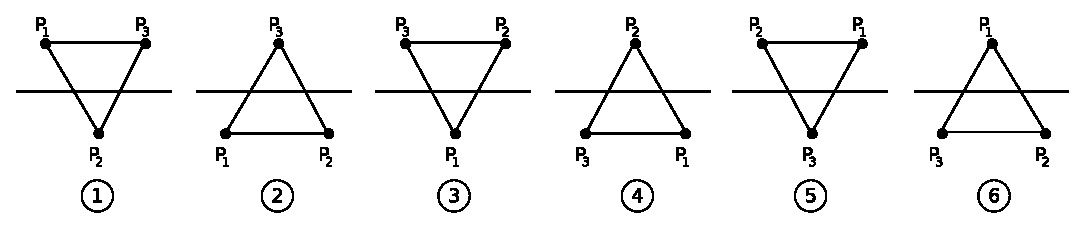
\includegraphics[width=400px]{pictures/faces_schnitte.eps}
    \caption{Ebene-Face Schnittm"oglichkeiten}
    \label{fig:faces_schnitte}
\end{figure}

Es k"onnen sechs verschiedene F"alle unterschieden werden. F"ur die
Fallunterscheidung signifikant sind die
\texttt{z}-Koordinaten der drei Vertices jedes Faces. Es wird gepr"uft, welcher
Vertex oberhalb und welcher unterhalb der Ebene liegt. Aus Symmetriegr"unden
k"onnen bei der weiteren Berechnung die F"alle \texttt{1} und \texttt{4},
\texttt{2} und \texttt{5} sowie \texttt{3} und \texttt{6} zusammengefasst
werden, da jeweils die gleichen Seiten des Face-Dreiecks geschnitten werden.\\
Um die genaue
Schnittkante zwischen dem Face und der Ebene zu berechnen wird bestimmt,
welche beiden Seiten des Faces geschnitten werden. Aus den daraus
resultierenden Schnittpunkten l"asst sich anschlie\ss end die
Schnittkante zusammensetzen.\\
Das bedeutet, dass f"ur jedes Face zweimal ein Schnittpunkt zwischen einer
Gerade und der aktuellen Ebene durchgef"uhrt werden muss.
Umgesetzt wird dies mit Hilfe einfacher Vektorgeometrie. Zur besseren
Veranschaulichung ist die Abbildung \ref{fig:sp_gerade_ebene} gegeben.

\begin{figure}[htbp]
    \centering
    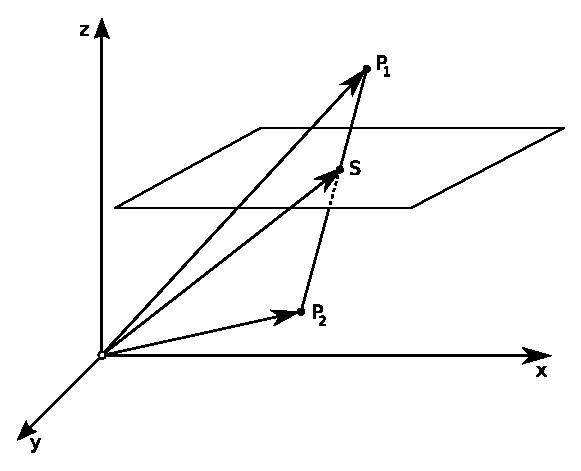
\includegraphics[width=300px]{pictures/sp_gerade_ebene.eps}
    \caption{Schnittpunkt von einer Geraden mit einer Ebene}
    \label{fig:sp_gerade_ebene}
\end{figure}

Exemplarisch soll sich hier auf eine Seite und deren Schnittpunkt mit einer
Ebene beschr"ankt werden.
Gegeben sind die Punkte $P_1$ und $P_2$ und gesucht ist
der Schnittpunkt $S$, wobei die \texttt{z}-Koordinate von $S$ durch die Ebene
bereits gegeben ist. Insbesondere sind folglich die \texttt{x}- und die
\texttt{y}-Koordinate von $S$ von Interesse.
Die Punkte k"onnen ebenso als Vektoren betrachtet werden,
so, wie in der Zeichnung angedeutet. Auch die Kante $\overrightarrow{P_2 P_1}$
selbst kann als
Vektor dargestellt werden durch
\begin{equation*}
    \overrightarrow{P_2 P_1} = P_1 - P_2
\end{equation*}
Da der Schnittpunkt offensichtlich auf diesem Vektor liegen muss, kann $S$
zun"achst wie folgt geschrieben werden:
\begin{equation*}
    S = \lambda \overrightarrow{P_2 P_1}
\end{equation*}
Dabei ist $\lambda$ ein Skalierungsfaktor f"ur den gilt
\begin{equation*}
    \lambda = \frac{z^* - z_2}{z_1 - z_2}
\end{equation*}
Der Wert $z^*$ stellt die gegebene \texttt{z}-Koordinate der betrachteten Ebene
dar und $z_1$ bzw. $z_2$ die \texttt{z}-Koordinaten der beiden Punkte $P_1$ und
$P_2$.
%mit $\lambda \in \[0,1\]$.

Des Weiteren muss ber"uchsichtigt werden, dass $S$ im Moment noch von
$P_2$ und nicht vom Ursprung ausgeht. Um die richtigen Koordinaten von $S$
zu erhalten muss zuletzt noch der Vektor $\vec{P_2}$ zu dem Ergebnis
hinzuaddiert werden, sodass sich f"ur die gesuchten \texttt{x}- und
\texttt{y}-Koordinaten des Schnittpunktes folgende Formeln aufstellen lassen:
\begin{align*}
    x_1^* &= \frac{z^* - z_2}{z_1 - z_2} (x_1 - x_2) + x_2 \\
    y_1^* &= \frac{z^* - z_2}{z_1 - z_2} (y_1 - y_2) + y_2
\end{align*}
Analog lassen sich die Koordinaten $x_2^*$ und $y_2^*$ des Schnittpunktes der
zweiten Kante
berechnen. Zum Schluss werden die Koordinaten aller Schnittkanten in einem
\texttt{edges}-Array gespeichert, wobei eine Kante immer aus vier Koordinaten
besteht,
die hintereinander in das Array eingetragen werden.\\
Mit den so berechneten Schnittkanten kann im Folgenden der Punkt in Polygon
Algorithmus im Zweidimensionalen angewandt werden.


\subsection{Punkt in Polgon - Algorithmus anwenden}

Durch die im vorherigen Abschnitt {\ref{sec:schnittkanten}} bestimmten
Schnittkanten zwischen der Ebene
und den betroffenen Faces kann im Folgenden der in Kapitel \ref{sec:pip_theo}
bereits theoretisch erl"auterte, zweidimensionale Punkt in Polygon - Algorithmus
angewandt werden.\\
Die \texttt{punktInPolygon}-Methode bekommt hierzu die Koordinaten des zu
testenden Voxels und ein Array mir allen Polygonkanten der Ebene "ubergeben.

\inputminted[linenos=true]{java}{code/PunktInPolygon.java}

Dabei muss f"ur jede Polygonkante gepr"uft werden, ob sie einen Schnittpunkt
mit dem Test-Strahl hat, oder nicht. Da jede Kante aus zwei Punkten, bzw.
vier Koordinaten besteht, werden diese zu Beginn aus dem \texttt{edges}-Array
geholt und zwischengespeichert.
Schlie\ss lich gibt es nur zwei relevante Zust"ande (innerhalb und au\ss erhalb)
die in einer Variable \texttt{inside} vom Typ \texttt{boolean} gespeichert
werden k"onnen.\\
Zur effizienteren Berechnung wird der Test-Strahl in Richtung der positiven
\texttt{x}-Achse geschossen.
Um nur die relevanten Kanten auf einen Schnittpunkt mit dem Strahl zu testen,
wird vorab gepr"uft, ob Anfangs- und Endpunkt der aktuellen Polygonkante beide
oberhalb oder beide unterhalb des Teststrahls liegen. Ist dies der Fall, so
liegt kein Schnittpunkt vor. Dabei wird die Annahme, dass ein Polygonvertex
infinitisimal "uber dem Test-Strahl liegt in Zeile 11 und 12 umgesetzt.
Einen Schnittpunkt kann es nur geben, wenn ein Punkt oberhalb und der andere
unterhalb des Strahls liegt, wobei dann die \texttt{x}-Koordinaten genauer
untersucht werden. Liegen beide Punkte rechts von dem zu pr"ufenden Punkt
(d.h. $x1>x$ und $x2>x$), so
schneidet die Kante den Strahl irgendwo und \texttt{inside} wechselt den Wert.
Sind die \texttt{x}-Koordinaten der beiden Punkte kleiner als \texttt{x}, dann
gibt es keinen Schnittpunkt. Liegt ein Punkt rechts und der andere links von
\texttt{x}, so muss berechnet werden, ob der Schnittpunkt rechts von dem
Textvoxel liegt. Ist dies der Fall, so wechselt \texttt{inside} erneut seinen
Wert.\cite[S. 51ff.]{skript_cg}
\\
Das Ergebnis des Punkt-in-Polygon-Algorithmus l"asst sich in Abbildung
\ref{fig:voxel_in_object} gut erkennen. Das erste Bild zeigt die mit Voxeln
gef"ullte Szene und im zweiten Bild sieht man alle Voxel, die innerhalb der
Schachfigur liegen.

\begin{figure}[htbp]
    \centering
    \includegraphics[width=250px]{pictures/voxel_in_object.png}
    \caption{Voxel in Objekt - Algorithmus}
    \label{fig:voxel_in_object}
\end{figure}



\section{Marching Cubes - Algorithmus}
\label{sec:mc_algo}

Der folgende Abschnitt beschreibt die Umsetzung des in Kapitel \ref{sec:mc_theo}
dargestellten Marching Cubes Algorithmus in Java, basierend auf einer
Implementation von Cory Gene Bloyd in C++. \cite{mc_algo}\\
Um  sp"ater zu bestimmen an welchen Stellen der Szene Schnee fallen kann, dient
dieser Algorithmus zun"achst als Grundlage, um die Oberfl"ache der Szene bzw.
der Objekte innerhalb der Szene nachzubilden.\\
Gegeben ist das aus Kapitel \ref{sec:voxel_fill} bekannte regelm"a\ss ige,
dreidimensionale Voxelgitter. Jeder Voxel enth"alt die Information, ob er
innerhalb oder au\ss erhalb eines Objektes liegt.
Es wird nun eine neue Oberfl"ache erstellt, indem man kubusweise durch das
Voxelgrid durchgeht, den jeweiligen W"urfel auf Schnittpunkte mit der
Objektoberfl"ache untersucht und die entsprechenden Dreiecke zeichnet.
Dabei k"onnen verschiedene F"alle auftreten. Die Objektoberfl"ache durchtrennt
den Kubus nicht, sie schneidet einen Vertex ab oder teilt ihn beliebig komplex
in Innen- und Au\ss enbereiche auf. Die Aufteilung richtet sich nach der Anzahl
und dem Index der innen- bzw. au\ss enliegenden Eckvoxeln des Kubus.
Insgesamt kann es 256 verschiedene F"alle geben, welche in Abbildung
\ref{fig:mc_possibilities} bereits illustriert wurden.\\
Die Bestimmung der Eckpunkte der zu zeichnenden Dreiecke richtet sich nach
der Anzahl und dem Index der geschnittenen W"urfelkanten. Liegt zum Beispiel
ein Voxel innerhalb eines Objekts und ein benachbarter Voxel au\ss erhalb, so
muss die Objektoberfl"ache einen Schnittpunkt mit der Kante zwischen diesen
beiden Voxeln haben. Die genaue Position des Schnittpunktes kann linear
interpoliert werden, worauf in diesem Fall allerdings nicht eingegangen wird.
Stattdessen wird stets der Kantenmittelpunkt als Schnittpunkt gew"ahlt.\\
%Anschlie\ss end wird in der \texttt{TriangleLookupTable} (TLT) nachgesehen,



\subsection{Imagin"aren Cube erstellen}

Der Marching Cubes Algorithmus geht jeden Voxel der Szene durch und bildet
mit diesem als Referenzvoxel
einen imagin"aren W"urfel.
Das bedeutet, dass die restlichen sieben Eckvoxel anhand des ersten bestimmt
werden.\\
Die Indizierung der Voxel von \texttt{v0} bis \texttt{v7} sowie der Kanten
von \texttt{e0} bis \texttt{e11} wie sie bei der Umsetzung des Algorithmus
verwendet werden, ist in Abbildung \ref{fig:cube} dargestellt.

\begin{figure}[htbp]
    \centering
    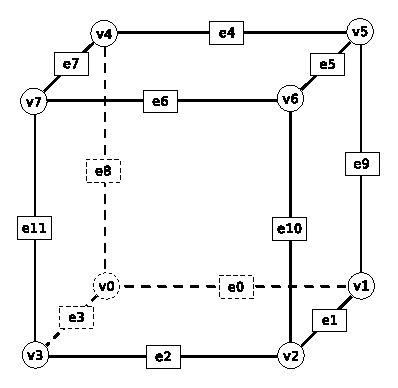
\includegraphics[width=200px]{pictures/cube.eps}
    \caption{Indizierung eines Marching Cubes}
    \label{fig:cube}
\end{figure}

Der Referenzvoxel ist dabei immer die hintere linke Ecke des Kubus. Arbeitet man
mit Vertices, so k"onnen die anderen Eckpunkte mit Hilfe eines Offsets
bestimmt werden. In diesem Fall hingegen werden die Nachbarschaftsbeziehungen
eines Voxels ausgenutzt um zu dem selben Ergebnis zu kommen.

\inputminted[linenos=true]{java}{code/Cube.java}

Wie in dem Codebeispiel zu sehen ist, werden alle acht W"urfelecken in einem
Voxel-Array gespeichert, wobei \texttt{cube[0]} der Referenzvoxel ist.


\subsection{Schnittkanten mit der Ebene bestimmen}

Um im Anschluss die Schnittkanten des W"urfels mit einem Objekt zu ermitteln
werden alle Eckpunkte darauf getestet ob sie innerhalb eines Objektes liegen
oder
Schnee beinhalten. Im zweiten Fall wird ein Voxel genauso behandelt wie im
ersten, da er dann bereits in der Schneedecke liegt, das bedeutet unterhalb der
Schneeoberfl"ache.

\inputminted[linenos=true]{java}{code/FlagIntex.java}

Ist der Test erfolgreich, so wird sich mit einem 8-Bit Index gemerkt, wobei
jedes Bit einem Eckvoxel entspricht.
Dies geschieht mit einer Bitshift-Operation der 1 um
die entsprechende Anzahl an Stellen nach links verschiebt.
Ist ein Voxel innenliegend, so wird das Bit auf 1 gesetzt, ansonsten bleibt es
0.\\
Dieser Teil l"asst sich am Besten anhand eines Beispiels erkl"aren. Es sei
der W"urfel aus Abbildung \ref{fig:cube_example} gegeben. Nun schneidet eine
Objektoberfl"ache
den Kubus derart, dass \texttt{cube[0]} und \texttt{cube[1]} (also \texttt{v0}
und \texttt{v1}) innerhalb des Objektes liegen.

\begin{figure}[htbp]
    \centering
    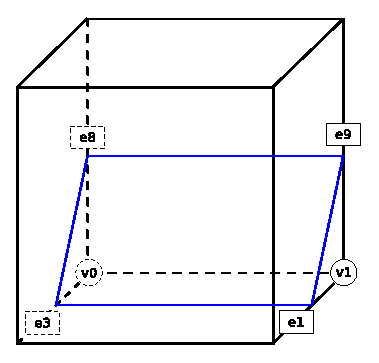
\includegraphics[width=200px]{pictures/cube_example.eps}
    \caption{Beispiel Cube}
    \label{fig:cube_example}
\end{figure}

Der \texttt{iFlagIndex} betr"agt folglich \texttt{0000 0011} in bin"arer oder
\texttt{3} in dezimaler Kodierung.
Als n"achstes wird in einer Tabelle bzw. einem Array nachgesehen, welche
W"urfelkanten von der Oberfl"ache bei gegebenem \texttt{iFlagIndex}
geschnitten werden.

\inputminted[linenos=true]{java}{code/EdgeFlags.java}

Dieses Array hei\ss t \texttt{CubeEdgeFlags}, hat
256 Eintr"age, entsprechend aller Schnittm"oglichkeiten und bildet den
8-Bit \texttt{iFlagIndex} auf eine 12-Bit kodierte Zahl mit dem Namen
\texttt{iEdgeFlags} ab.

\inputminted[linenos=true]{java}{code/CubeEdgeFlags.java}

Auch hier entpricht jedes Bit einer bestimmten Kante.
Ein Bit ist auf 1 gesetzt, wenn die Objektoberfl"ache die Kante schneidet und
auf 0, falls es
keinen Schnittpunkt gibt. Ist \texttt{iEdgeFlags == 0}, so wird keine der
W"urfelkanten geteilt und es
kann mit dem n"achsten Kubus fortgefahren werden.\\
Bezogen auf das obere Beispiel bedeutet dies, dass
\texttt{iEdgeFlags[3] = 0011 0000 1010} in Bin"ar- oder \texttt{0x30a} in
Hexadezimalform.
Das hei\ss t, es werden die Kanten \texttt{e1}, \texttt{e3}, \texttt{e8} und
\texttt{e9} von der Objektoberfl"ache geschnitten, wie auch in Abbildung
\ref{fig:cube_example} zu sehen ist.\\
Anschlie\ss end werden die Koordinaten der Schnittpunkte auf den jeweiligen
Kanten berechnet und in dem zw"olfelementigen \texttt{Vertex}-Array
\texttt{edgeVertex} gespeichert.
Dazu betrachtet man jede Kante und pr"uft, ob in \texttt{iEdgeFlags} an der
entsprechenden Stelle eine \texttt{1} steht. Ist dies der Fall, so folgt
eine Schnittpunktberechnung durch lineare Interpolation. Es wird
bei den waagerechten Kanten (\texttt{e0} bis \texttt{e7}), wie in
Abschnitt \ref{sec:voxel} bereits angek"undigt, der Einfachheit halber von
dem Mittelpunkt einer Kante als Schnittpunkt ausgegangen.
Lediglich die \texttt{z}-Koordinaten der senkrechten W"urfelkanten
(\texttt{e8} bis \texttt{e11}) weichen von
der Mitte ab und richten sich nach
dem \texttt{Density}-Wert des zugeh"origen, unteren Voxels.\\
Der folgende Codeauschnitt verdeutlicht das oben beschriebene Vorgehen.

\inputminted[linenos=true]{java}{code/Intersection.java}

Die Koordinaten eines Schnittpunktes lassen sich mit Hilfe von drei Hilfsarrays
berechnen. Zun"achst wird im \texttt{EDGE\_CONNECTION}-Array nachgesehen,
welche beiden Voxel die aktuelle Kante verbindet. Danach wird die Entfernung
des Schnittpunktes vom Referenzvoxel durch das
\texttt{VOXEL\_OFFSET}-Array bestimmt. Damit der Vertex an der richtigen Stelle
platziert wird gibt \texttt{EDGE\_DIRECTION} die Richtung der
Kante an. Der Wert \texttt{0.5f} bedeutet, dass der Kantenmittelpunkt als
Schnittpunkt gew"ahlt wird. \texttt{scale} skaliert schlie\ss lich die
Positionierung in
Abh"angigkeit zur Granularit"at des \texttt{Voxel}-Gitters
($\texttt{scale} = \frac{1}{\texttt{STEPS}}$).\\

Zur besseren Visualisierung werden neben den Schnittpunkten auch
die Einheitsnormalen an eben diesen Punkten berechnet.


\subsection{\texttt{TriangleLookupTable}}

Nachdem alle Schnittpunkte eines Kubus mit der Objektoberfl"ache berechnet
wurden m"ussen diese noch in korrekter Reihenfolge zu Dreiecken bzw.
\texttt{Faces} verbunden werden.
Hierzu wird erneut ein Array verwendet, das den selben \texttt{iFlagIndex}
verwendet wie zuvor \texttt{CubeEdgeFlags} und es erlaubt die
\texttt{Vertex}-Sequenz zur Darstellung der angen"ahrten Oberfl"ache
nachzuschlagen. Das \texttt{TriangleLookupTable}-Array ist
zweidimensional und besteht aus \texttt{256 x 16} Eintr"agen, da es
\texttt{256} Teilungsm"oglichkeiten und pro Cube bis zu f"unf \texttt{Faces}
gibt. Die \texttt{TriangleLookupTable} hat die folgende Form.

\inputminted[linenos=true]{java}{code/TriangleLookupTable.java}

Dabei steht die \texttt{-1} f"ur einen invaliden Eintrag und zeigt an, dass
der Algorithmus f"ur diesen Cube an dieser Stelle abgebrochen werden kann
(siehe Zeile 4-5 im unteren Code-Beispiel).\\

\inputminted[linenos=true]{java}{code/UseTLT.java}

Folglich werden die bis zu f"unf M"oglichkeiten durchgegangen. Soll ein
\texttt{Face} sp"ater gezeichnet werden, so wird auf die
Vertices des \texttt{edgeVertex}-Arrays in richtiger Reihenfolge
zugegriffen und diese entgegen dem
Uhrzeigersinn in einer Instanzvariable \texttt{faces} abgespeichert.\\
Erneut bezogen auf den obigen Beispielfall liefert der Aufruf
\texttt{TriangleLookupTable[3]} die Zeile:
\\
\\
\texttt{\{1, 8, 3, 9, 8, 1, -1, -1, -1, -1, -1, -1, -1, -1, -1, -1\}}
\\
\\
Das bedeutet, dass f"ur diesen Cube zwei \texttt{Faces} gezeichnet werden
m"ussen. Zum einen bestehend aus den Vertices mit den Indices
\texttt{(1, 8, 3)} und zum anderen
aus \texttt{(9, 8, 1)}.

\subsection{Ergebnis}




\section{Schneedecke}


\subsection{Schnee von oben}


\subsection{Schnee von der Seite}


\subsection{Schneestabilit"at}

\cite{fallen_snow}


%%%%%%% REFLEXION %%%%%%%%

\chapter{Reflexion}

\section{Zusammenfassung}

\section{Fazit und Ausblick}


% DON'T set \bibliographystyle here -- use the documentclass option instead
\bibliography{papers}

\closing %%%%%%%%%%%%%%%%%%%%%%%%%%%%%%

\end{document}
